%%
%%
%% proposition_software.tex for thesis in /doctorat/these/tex
%%
%% Made by Philippe THIERRY
%% Login   <Philippe THIERRYreseau-libre.net>
%%
%% Started on  Thu Mar 18 17:20:20 2010 Philippe THIERRY
%% Last update mer. 13 juil. 2011 14:24:17 CEST Philippe THIERRY
%%

\chapter{Derivating formal model to software architecture}

\doMinitoc

\section{On the deployment of a MILS-compliant architecture}

\subsection{Integration of a separation-kernel based architecture}

\subsection{Scheduling partitions}

\section{Integrating a Role-Based access control of partitions}

\section{Impact of real-time integration}

\subsection{Defining a real-time compliant security levels distribution}

\subsection{Impact on the real-time and security hypothesis}

\section{About the hardware plateform selection}

\subsection{The QorIQ MPSoC familly}

\paragraph{}
QorIQ MPSoC familly is an interesting choice for a real-time and secure system for critical network
flow management. As shown in Figure \ref{fig:qoriq2040bd}, this architecture has various interesting
elements:
\begin{itemize}
\item Multiple separated network controlers
\item Separated multiple DMA controlers, which permit to separate NIC control plane from DMA control plane
\item QorIQ-specific {\it I/OMMU}, which is theoricaly able to control device to memory and device
to device access. Nevertheless, such module should be validated in order to be considered as a
trustworthy element
\item multi-level memory management, with unshared L1 and L2 caches
\item \FIXME{scratchpad capacities - check how to use it}
\item Internal NoC which reduce central interconnect bottle-neck, yet not described.
\end{itemize}

\begin{figure}[ht]
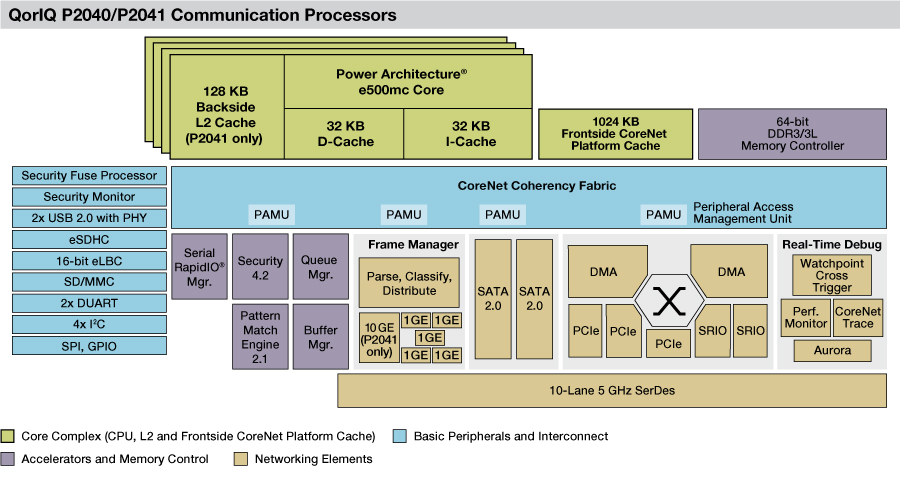
\includegraphics[width=17cm]{figures/P2040_BD}
\caption{Freescale p2040 QorIQ bloc diagram\label{fig:qoriq2040bd}}
\end{figure}

\subsection{Missing hardware elements for a complete secure \& real-time system}


%\chapter{D�fining a real-time and secure software plateform}
%
%
%\section{D�fining an optimized scheduling policy for network processing}
%
%\subsection{About the synchronous network flows processing}
%
%Utilisation de threads kernel g�r�s comme des taches temps r�elles
%
%\subsection{About the asyncrhonous network flows}
%
%Cas des protocoles CSMA/CD, CSMA/CA. Ordonnancement de type temps r�el 'souple'.
%
%\subsection{Security policy management and data flow paritioning}
